\part{Basic Theories}

\chapter{Fundamentals of Generative Adversarial Networks}
\section{Definition and Background of GANs}
Generative Adversarial Networks (GANs)~\cite{goodfellow2014generative} are one of the most groundbreaking advancements in machine learning, particularly in the field of unsupervised learning. Introduced by Ian Goodfellow~\cite{goodfellow2014generative} and his colleagues in 2014, GANs represent a novel approach to generating data that looks similar to the data the model was trained~\cite{creswell2018generative,metz2016unrolled}.

\begin{figure}[htbp]
    \centering
    \includegraphics[width=0.8\textwidth]{figs/gan_history.pdf}
    \caption{Evolution of GAN performance from 2014 to 2018 and 2024. The results for 2014 to 2018 are based on the demonstration by Goodfellow~\cite{goodfellow2014generative} at the International Conference on Learning Representations (ICLR) 2019 invited talk, showcasing the rapid advancements in GAN quality over the years~\cite{radford2015unsupervised, liu2016coupled, karras2017progressive, karras2019style}. The figure of 2024 from ISFB-GAN~\cite{peng2024isfb}.}
\end{figure}

\subsection{Definition of GAN}
At its core, a GAN consists of two neural networks, referred to as the \textbf{generator} and the \textbf{discriminator}, which are pitted against each other in a zero-sum game~\cite{goodfellow2014generative,wang2017generative}. The generator attempts to create fake data that resembles the real data, while the discriminator tries to distinguish between real and fake data~\cite{aggarwal2021generative, gui2021review}. These two networks are trained simultaneously:

\begin{itemize}
    \item \textbf{Generator:} A neural network that takes random noise as input and attempts to generate data that mimics the real dataset~\cite{goodfellow2014generative}.
    \item \textbf{Discriminator:} Another neural network that evaluates the data and determines whether the input data is from the real dataset or generated by the generator~\cite{goodfellow2014generative,gui2021review}.
\end{itemize}

The goal is to train the generator to the point where the discriminator can no longer reliably distinguish between real and fake data.

\subsection{Historical Development of GANs}
The journey of GANs began with the work of Ian Goodfellow in 2014~\cite{goodfellow2014generative}, but the concepts that led to GANs can be traced back to earlier advancements in deep learning and neural networks~\cite{gui2021review}. Here's a brief overview of the major milestones in the history of GANs:

\begin{itemize}
    \item \textbf{2014:} GAN was introduced by Ian Goodfellow. In the original paper, the authors proposed a novel framework for generative models~\cite{goodfellow2014generative}.
    \item \textbf{2016:} The introduction of techniques like Wasserstein GAN (WGAN)~\cite{arjovsky2017wasserstein} helped to improve the stability of training, which was a significant issue in the early implementations~\cite{gui2021review}.
    \item \textbf{2017:} Progressive Growing of GANs (PGGANs)~\cite{karras2017progressive} was proposed, enabling the generation of high-resolution images.
    \item \textbf{2018:} GANs were used to generate high-quality human faces~\cite{gui2021review,park2019semantic} (e.g., StyleGAN~\cite{karras2019style}).
    \item \textbf{2019:} BigGAN~\cite{brock2018large} introduced large-scale training and incorporated self-attention mechanisms, achieving significant improvements in image quality and diversity. It set a new benchmark for high-resolution image generation.
    \item \textbf{2020:} StyleGAN2~\cite{karras2020analyzing} enhanced its predecessor by improving normalization techniques and architecture design, leading to more realistic images and reducing artifacts in the generated outputs.
    \item \textbf{2021:} GauGAN~\cite{park2019semantic} demonstrated the ability of GANs to transform simple sketches into photorealistic images, showcasing the strength of GANs in semantic image synthesis. It became a powerful tool for creative applications.
    \item \textbf{2022:} StyleGAN3~\cite{karras2021alias} addressed aliasing artifacts present in earlier versions and improved the spatial consistency of generated images under transformations, achieving higher-quality and more stable outputs.
    \item \textbf{2023:} GigaGAN~\cite{kang2023scaling} introduced a scalable architecture capable of generating ultra-high-resolution images with improved quality and significantly faster generation times, advancing the frontier of GAN research.
    \item \textbf{2024:} GAN (SparseGAN~\cite{zhou2020sparse}) focused on reducing computational overhead while maintaining high-quality image generation. By leveraging sparsity in network design, it provided a more efficient approach to GAN training and deployment.
\end{itemize}

\subsection{Comparison Between GAN and Traditional Generative Models}
To understand the significance of GANs, it's important to compare them with more traditional generative models like Variational Autoencoders (VAEs)~\cite{kingma2013auto,kingma2019introduction} and Restricted Boltzmann Machines (RBMs)~\cite{ackley1985learning,nair2010rectified}.

\subsubsection{Traditional Generative Models}
Before the advent of GANs, most generative models relied on certain assumptions or simplifications in modeling the data distribution~\cite{aggarwal2021generative}. For instance:

\begin{itemize}
    \item \textbf{Restricted Boltzmann Machines (RBM):} RBMs are energy-based models that learn a probability distribution~\cite{ramberg1979probability} over input data. They were widely used for dimensionality reduction~\cite{van2009dimensionality} and pretraining of deep networks~\cite{nair2010rectified,erhan2010does}.
    \item \textbf{Variational Autoencoders (VAE):} VAEs aim to learn latent representations of data by optimizing the Evidence Lower Bound (ELBO)~\cite{hoffman2016elbo} and using a combination of an encoder and decoder architecture~\cite{kingma2019introduction}.
\end{itemize}

While these methods were effective in some tasks, they have notable limitations:

\begin{itemize}
    \item VAEs often produce blurry outputs due to their reliance on the Gaussian distribution~\cite{goodman1963statistical} in latent space~\cite{hoff2002latent}.
    \item RBMs have limitations in terms of scalability and convergence~\cite{nair2010rectified}.
\end{itemize}

\subsubsection{Advantages of GANs over Traditional Models}
GANs differ from traditional generative models primarily in their adversarial training approach~\cite{goodfellow2014generative,creswell2018generative,aggarwal2021generative,gui2021review}. Instead of relying on a fixed probability distribution, GANs employ the generator and discriminator in a game-theoretic setup~\cite{goodfellow2014generative,aggarwal2021generative}. The advantages of GANs include:

\begin{itemize}
    \item \textbf{High-quality data generation:} GANs often generate sharper and more realistic outputs than VAEs~\cite{wang2017generative}.
    \item \textbf{Flexibility:} GANs do not require explicit probability distributions for their outputs, making them more flexible in generating various types of data~\cite{kazeminia2020gans}.
    \item \textbf{Adversarial training:} The discriminator provides a continuous feedback loop to the generator, leading to improved performance over time~\cite{aggarwal2021generative}.
\end{itemize}

\section{Understanding GAN with Python: A Simple Example}
In this section, we will implement a simple GAN using PyTorch~\cite{paszke2019pytorch}, a popular deep learning framework. For the purpose of illustration, let's consider a basic problem: generating a distribution that mimics the behavior of a 1D Gaussian distribution~\cite{stevens2020deep}.

First, we need to set up the environment and libraries:

\begin{lstlisting}[style=cmd]
pip install torch torchvision matplotlib numpy
\end{lstlisting}

Next, we implement the generator and discriminator models:

\subsection{Step 1: Import Necessary Libraries}
We begin by importing the required libraries:

\begin{lstlisting}[style=python]
import torch
import torch.nn as nn
import torch.optim as optim
import numpy as np
import matplotlib.pyplot as plt
\end{lstlisting}

\subsection{Step 2: Define the Generator and Discriminator}
The generator network will take a random noise vector~\cite{gui2021review} as input and output a single scalar. The discriminator, on the other hand, will take a scalar and attempt to classify it as either real (coming from a true Gaussian distribution) or fake (generated by the generator).

\begin{lstlisting}[style=python]
# Define the Generator model
class Generator(nn.Module):
    def __init__(self, input_size, hidden_size, output_size):
        super(Generator, self).__init__()
        self.net = nn.Sequential(
            nn.Linear(input_size, hidden_size),
            nn.ReLU(),
            nn.Linear(hidden_size, output_size)
        )

    def forward(self, x):
        return self.net(x)

# Define the Discriminator model
class Discriminator(nn.Module):
    def __init__(self, input_size, hidden_size, output_size):
        super(Discriminator, self).__init__()
        self.net = nn.Sequential(
            nn.Linear(input_size, hidden_size),
            nn.ReLU(),
            nn.Linear(hidden_size, output_size),
            nn.Sigmoid()
        )

    def forward(self, x):
        return self.net(x)
\end{lstlisting}

\subsection{Step 3: Training the GAN}
Now that we have our models defined, we will train the GAN. The generator will learn to generate samples that match a target 1D Gaussian distribution~\cite{goodman1963statistical}, while the discriminator will try to distinguish between real and fake samples~\cite{goodfellow2014generative}.

First, let's initialize the models and the optimizers:

\begin{lstlisting}[style=python]
# Hyperparameters
input_size = 1
hidden_size = 128
output_size = 1
learning_rate = 0.0002

# Create the models
generator = Generator(input_size, hidden_size, output_size)
discriminator = Discriminator(output_size, hidden_size, 1)

# Optimizers
optimizer_g = optim.Adam(generator.parameters(), lr=learning_rate)
optimizer_d = optim.Adam(discriminator.parameters(), lr=learning_rate)

# Loss function
loss_function = nn.BCELoss()
\end{lstlisting}

We'll generate real data from a Gaussian distribution and train the discriminator and generator iteratively:

\begin{lstlisting}[style=python]
# Training loop
num_epochs = 5000
real_data_mean = 4
real_data_stddev = 1.25

for epoch in range(num_epochs):
    # Train Discriminator: maximize log(D(x)) + log(1 - D(G(z)))
    real_data = torch.randn(32, 1) * real_data_stddev + real_data_mean
    fake_data = generator(torch.randn(32, 1)).detach()

    real_labels = torch.ones(32, 1)
    fake_labels = torch.zeros(32, 1)

    d_loss_real = loss_function(discriminator(real_data), real_labels)
    d_loss_fake = loss_function(discriminator(fake_data), fake_labels)
    d_loss = d_loss_real + d_loss_fake

    optimizer_d.zero_grad()
    d_loss.backward()
    optimizer_d.step()

    # Train Generator: minimize log(1 - D(G(z))) or maximize log(D(G(z)))
    noise = torch.randn(32, 1)
    g_loss = loss_function(discriminator(generator(noise)), real_labels)

    optimizer_g.zero_grad()
    g_loss.backward()
    optimizer_g.step()

    if epoch % 1000 == 0:
        print(f'Epoch [{epoch}/{num_epochs}], d_loss: {d_loss.item():.4f}, g_loss: {g_loss.item():.4f}')
\end{lstlisting}
In this code, the generator is trained to improve its ability to fool the discriminator by producing outputs that resemble the real data distribution. The discriminator, in turn, is trained to distinguish between real and fake samples.

\section{Summary}
In this chapter, we explored the basic concepts of GANs, including their definition, historical development, and advantages over traditional generative models~\cite{goodfellow2014generative,gui2021review}. We also implemented a simple GAN using PyTorch to generate a 1D Gaussian distribution, providing a practical example for beginners to understand how GANs work. By progressively refining both the generator and discriminator, the GAN is able to learn to produce realistic data~\cite{kazeminia2020gans}.










\section{GAN's Basic Structure}
Generative Adversarial Networks (GANs) are a class of machine learning frameworks designed to generate data similar to a given dataset. GANs consist of two primary components: the Generator and the Discriminator, both of which are neural networks that compete against each other in a zero-sum game~\cite{goodfellow2014generative,aggarwal2021generative}. This section will explain each component in detail and describe how they interact with each other.

\subsection{Generator}
The Generator is responsible for generating synthetic data that resembles real data from the dataset. Its goal is to learn the distribution of the real data and produce samples that the Discriminator cannot distinguish from real samples.

The Generator starts with random noise, typically drawn from a Gaussian or uniform distribution, and transforms it into data (e.g., an image) using a series of neural network layers~\cite{goodfellow2014generative}. Initially, the Generator's output will not resemble real data, but as it gets trained, it gradually improves.

\textbf{Example of a Generator's forward pass in PyTorch:}

\begin{lstlisting}[style=python]
import torch
import torch.nn as nn

class Generator(nn.Module):
    def __init__(self, input_dim, output_dim):
        super(Generator, self).__init__()
        self.model = nn.Sequential(
            nn.Linear(input_dim, 128),   # Input layer (noise)
            nn.ReLU(),
            nn.Linear(128, 256),         # Hidden layer
            nn.ReLU(),
            nn.Linear(256, output_dim),  # Output layer (generated data)
            nn.Tanh()                    # Activation function for image generation
        )

    def forward(self, x):
        return self.model(x)

# Example usage:
noise = torch.randn((1, 100))  # 100-dimensional random noise
gen = Generator(100, 784)      # 784 = 28x28 pixels (for image generation)
generated_data = gen(noise)
print(generated_data.shape)    # Should output: torch.Size([1, 784])
\end{lstlisting}

In the above example, the Generator network consists of several fully connected (linear) layers with ReLU activations, except for the output layer where we use a Tanh activation function. Tanh is commonly used when generating image data because it restricts the output to values between -1 and 1, matching the normalized pixel values of images.

\subsection{Discriminator}
The Discriminator's role is to distinguish between real data (from the dataset) and the fake data produced by the Generator. It outputs a probability indicating whether it believes a given sample is real or fake~\cite{goodfellow2014generative}. Its objective is to maximize the accuracy of distinguishing between real and fake data.

\textbf{Example of a Discriminator's forward pass in PyTorch:}

\begin{lstlisting}[style=python]
class Discriminator(nn.Module):
    def __init__(self, input_dim):
        super(Discriminator, self).__init__()
        self.model = nn.Sequential(
            nn.Linear(input_dim, 256),   # Input layer (real or fake data)
            nn.LeakyReLU(0.2),
            nn.Linear(256, 128),         # Hidden layer
            nn.LeakyReLU(0.2),
            nn.Linear(128, 1),           # Output layer (real/fake probability)
            nn.Sigmoid()                 # Sigmoid function to get probability
        )

    def forward(self, x):
        return self.model(x)

# Example usage:
disc = Discriminator(784)  # Assuming the input is a 28x28 image flattened to 784 dimensions
real_data = torch.randn((1, 784))  # A real data sample from the dataset
discriminator_output = disc(real_data)
print(discriminator_output)  # Outputs a probability value between 0 and 1
\end{lstlisting}

The Discriminator network is also a fully connected neural network, but its final layer uses a Sigmoid activation function, which outputs a value between 0 and 1, representing the probability that the input is real.

\subsection{The Adversarial Game Between Generator and Discriminator}
GANs are based on a two-player game between the Generator and the Discriminator. The Generator tries to fool the Discriminator by producing data that is as close as possible to real data. Meanwhile, the Discriminator is trained to correctly classify real and fake data~\cite{goodfellow2014generative}.

The training process is adversarial, meaning the Generator improves by learning how to trick the Discriminator, and the Discriminator improves by becoming better at spotting fake data.

\subsubsection{Loss Functions}
The standard loss functions for GANs are:

\textbf{Generator Loss}: The Generator aims to minimize the following loss function~\cite{goodfellow2014generative}:
  \[
  \mathcal{L}_{G} = -\log(D(G(z)))
  \]
  Here, \( G(z) \) represents the fake data generated from noise \( z \), and \( D(G(z)) \) is the Discriminator's estimate of the probability that the fake data is real. The Generator wants to maximize this probability.

\textbf{Discriminator Loss}: The Discriminator aims to maximize the following loss function:
  \[
  \mathcal{L}_{D} = -\left( \log(D(x)) + \log(1 - D(G(z))) \right)
  \]
  Here, \( D(x) \) is the Discriminator's estimate that a real sample \( x \) is real, and \( D(G(z)) \) is its estimate that the fake data is real. The Discriminator tries to correctly classify both real and fake data~\cite{kazeminia2020gans}.

\textbf{Example of the training loop in PyTorch:}

\begin{lstlisting}[style=python]
# Hyperparameters
lr = 0.0002
epochs = 10000

# Instantiate models
gen = Generator(input_dim=100, output_dim=784)
disc = Discriminator(input_dim=784)

# Loss and optimizers
criterion = nn.BCELoss()
optimizer_gen = torch.optim.Adam(gen.parameters(), lr=lr)
optimizer_disc = torch.optim.Adam(disc.parameters(), lr=lr)

for epoch in range(epochs):
    # Train Discriminator
    optimizer_disc.zero_grad()

    # Real data
    real_data = torch.randn((64, 784))  # Batch of real data
    real_labels = torch.ones((64, 1))   # Label = 1 for real data
    output_real = disc(real_data)
    loss_real = criterion(output_real, real_labels)

    # Fake data
    noise = torch.randn((64, 100))      # Batch of noise
    fake_data = gen(noise)              # Generated fake data
    fake_labels = torch.zeros((64, 1))  # Label = 0 for fake data
    output_fake = disc(fake_data.detach())
    loss_fake = criterion(output_fake, fake_labels)

    # Total Discriminator loss and backpropagation
    loss_disc = loss_real + loss_fake
    loss_disc.backward()
    optimizer_disc.step()

    # Train Generator
    optimizer_gen.zero_grad()
    
    # Generate fake data again
    output_fake_for_gen = disc(fake_data)
    loss_gen = criterion(output_fake_for_gen, real_labels)  # We want the generator to fool the discriminator

    # Generator backpropagation
    loss_gen.backward()
    optimizer_gen.step()

    if epoch % 1000 == 0:
        print(f'Epoch [{epoch}/{epochs}], Loss D: {loss_disc.item()}, Loss G: {loss_gen.item()}')
\end{lstlisting}

In this code, both the Generator and Discriminator are trained alternately. First, the Discriminator is trained to distinguish between real and fake data. Then, the Generator is updated to produce better fake data that fools the Discriminator.

\subsection{Visualization of the GAN Structure}
Here is a simple tree-like representation of the GAN structure using \texttt{tikzpicture}~\cite{kottwitz2023latex}:

\begin{center}
\begin{tikzpicture}
  [scale=1, every node/.style={scale=1}, 
  block/.style={rectangle, draw, fill=blue!20, text centered, minimum height=3em},
  arrow/.style={->, thick}]

  % Nodes
  \node[block] (noise) {Noise (z)};
  \node[block, right=of noise] (gen) {Generator (G)};
  \node[block, right=of gen] (fake) {Fake Data};
  \node[block, below=of fake] (real) {Real Data};
  \node[block, right=of fake] (disc) {Discriminator (D)};
  \node[block, right=of disc] (output) {Real or Fake};

  % Arrows
  \draw[arrow] (noise) -- (gen);
  \draw[arrow] (gen) -- (fake);
  \draw[arrow] (real) -- (disc);
  \draw[arrow] (fake) -- (disc);
  \draw[arrow] (disc) -- (output);
\end{tikzpicture}
\end{center}

Generative Adversarial Networks (GANs) are composed of two primary components (as shown Fig \ref{fig:gan_basic_architecture}): a \textbf{Generator} and a \textbf{Discriminator}. These two networks work in opposition to each other to achieve a common goal, generating realistic data.

\begin{itemize}
    \item \textbf{Generator:}
    The Generator takes random noise as input and transforms it into synthetic data that resembles real samples. Its objective is to learn the data distribution and produce outputs that are indistinguishable from the real data. Over the course of training, the Generator improves by learning to ``fool'' the Discriminator.
    
    \item \textbf{Discriminator:}
    The Discriminator acts as a binary classifier, distinguishing between real data samples (from the dataset) and fake data samples (produced by the Generator). Its goal is to maximize its ability to correctly classify inputs as real or fake. 
\end{itemize}

The training process of a GAN is based on a minimax optimization game, where the Generator minimizes the classification performance of the Discriminator, while the Discriminator maximizes its classification accuracy. This dynamic adversarial process leads to the Generator creating more realistic data over time, eventually achieving a balance where the Discriminator can no longer reliably distinguish real from fake samples.

\begin{figure}[htbp]
    \centering
    \includegraphics[width=0.8\textwidth]{figs/gan_basic.pdf}
    \caption{The basic architecture of a Generative Adversarial Network (GAN). The Generator creates fake images from random noise, while the Discriminator evaluates images to determine whether they are real or fake. Both networks are trained adversarially to improve the quality of the generated samples.}
    \label{fig:gan_basic_architecture}
\end{figure}


\section{GAN's Objective Function and Optimization}
Generative Adversarial Networks (GANs) are an essential tool for generating synthetic data, and understanding their underlying objective functions is crucial~\cite{kazeminia2020gans}. In this section, we will explore the key objective functions involved in training GANs, with detailed examples and Python code using PyTorch.

\subsection{Binary Cross-Entropy Loss}
In a standard GAN, the generator and discriminator have competing objectives~\cite{goodfellow2014generative}, which can be defined using binary cross-entropy loss~\cite{ho2019real}.

The generator \(G\) tries to generate data that resembles the true data distribution, while the discriminator \(D\) aims to distinguish between real data and fake data generated by \(G\).

The loss for the discriminator can be defined as:
\[
\mathcal{L}_D = - \mathbb{E}_{x \sim p_{data}}[\log D(x)] - \mathbb{E}_{z \sim p_z}[\log (1 - D(G(z)))]
\]
Here, \(x \sim p_{data}\) represents samples from the real data distribution, and \(z \sim p_z\) are random noise vectors input to the generator~\cite{aggarwal2021generative}.

For the generator, the objective is to maximize the discriminator's error in classifying fake samples:
\[
\mathcal{L}_G = - \mathbb{E}_{z \sim p_z}[\log D(G(z))]
\]
This is also referred to as minimizing the negative log-likelihood~\cite{pinheiro1995approximations} of fooling the discriminator.

\begin{lstlisting}[style=python]
import torch
import torch.nn as nn
import torch.optim as optim

# Define the Discriminator model
class Discriminator(nn.Module):
    def __init__(self):
        super(Discriminator, self).__init__()
        self.main = nn.Sequential(
            nn.Linear(784, 512),
            nn.LeakyReLU(0.2),
            nn.Linear(512, 256),
            nn.LeakyReLU(0.2),
            nn.Linear(256, 1),
            nn.Sigmoid()
        )

    def forward(self, x):
        return self.main(x)

# Define the Generator model
class Generator(nn.Module):
    def __init__(self):
        super(Generator, self).__init__()
        self.main = nn.Sequential(
            nn.Linear(100, 256),
            nn.ReLU(),
            nn.Linear(256, 512),
            nn.ReLU(),
            nn.Linear(512, 784),
            nn.Tanh()
        )

    def forward(self, x):
        return self.main(x)

# Instantiate models
D = Discriminator()
G = Generator()

# Binary Cross-Entropy loss and optimizers
criterion = nn.BCELoss()
optimizer_D = optim.Adam(D.parameters(), lr=0.0002)
optimizer_G = optim.Adam(G.parameters(), lr=0.0002)

# Labels for real and fake data
real_label = torch.ones(64, 1)
fake_label = torch.zeros(64, 1)

# Example training step
for epoch in range(epochs):
    # Train the Discriminator
    optimizer_D.zero_grad()
    
    # Real data loss
    real_data = torch.randn(64, 784)  # Random real data for demonstration
    output = D(real_data)
    loss_real = criterion(output, real_label)
    
    # Fake data loss
    noise = torch.randn(64, 100)
    fake_data = G(noise)
    output = D(fake_data.detach())
    loss_fake = criterion(output, fake_label)
    
    # Total discriminator loss and backward
    loss_D = loss_real + loss_fake
    loss_D.backward()
    optimizer_D.step()
    
    # Train the Generator
    optimizer_G.zero_grad()
    output = D(fake_data)
    loss_G = criterion(output, real_label)
    
    loss_G.backward()
    optimizer_G.step()
\end{lstlisting}

\subsection{JS Divergence and KL Divergence}
A fundamental aspect of GANs is their reliance on the Jensen-Shannon (JS) divergence~\cite{gomez2000analysis} to measure the difference between the real data distribution and the distribution generated by \(G\). The JS divergence is a symmetrized and smoothed version of the Kullback-Leibler (KL) divergence~\cite{hershey2007approximating}, which is defined as:
\[
D_{KL}(P || Q) = \sum_{i} P(i) \log \left( \frac{P(i)}{Q(i)} \right)
\]
The KL divergence is non-symmetric and becomes infinite if there are samples that exist in \(P\) but not in \(Q\). This limitation can cause instability in GAN training~\cite{goodfellow2014generative}.

The JS divergence addresses this issue by computing the average between the real and fake distributions:
\[
JS(P || Q) = \frac{1}{2} D_{KL}(P || M) + \frac{1}{2} D_{KL}(Q || M)
\]
where \(M = \frac{1}{2}(P + Q)\) is the mixture distribution. GANs implicitly minimize the JS divergence between the real and generated data distributions during training.

\section{Training and Challenges of GANs}
Training GANs is challenging due to several issues, including mode collapse, vanishing gradients, and instability. Let's explore these problems and discuss how to mitigate them.

\subsection{Mode Collapse}
Mode collapse~\cite{srivastava2017veegan} occurs when the generator produces limited varieties of samples, even though the training data is diverse. In this situation, the generator might map multiple input noise vectors \(z\) to the same output, causing a lack of diversity in the generated data~\cite{thanh2020catastrophic}.

For example, suppose the real data consists of different images of digits (e.g., 0-9), but the generator only produces images of the digit '5'. This is mode collapse.

One common technique to mitigate mode collapse is to use \textbf{Mini-batch Discrimination}, where the discriminator looks at small batches of data instead of individual samples~\cite{thanh2020catastrophic}. This allows the discriminator to detect when the generator is producing similar outputs for different inputs.

\subsection{Vanishing Gradient and Instability}
Another challenge in GAN training is vanishing gradients~\cite{hochreiter1998vanishing}. If the discriminator becomes too strong, the generator may receive extremely small gradient updates, making it difficult to improve~\cite{hanin2018neural}.

This problem can be mitigated using techniques such as:
\begin{itemize}
    \item \textbf{Label Smoothing}: Instead of using binary labels (0 and 1), use slightly smoothed labels like 0.9 for real data and 0.1 for fake data. This helps the discriminator avoid becoming too confident and dominating the training process~\cite{muller2019does}.
    \item \textbf{Batch Normalization}: Adding batch normalization layers to the generator and discriminator helps stabilize the training process by normalizing activations and preventing exploding or vanishing gradients~\cite{santurkar2018does,bjorck2018understanding}.
    \item \textbf{Improved Loss Functions}: Using alternative loss functions such as the \textbf{Wasserstein loss}~\cite{frogner2015learning} can lead to more stable training and better convergence. The \textbf{Wasserstein loss} will be discussed in more detail in a later section.
\end{itemize}

\subsection{Techniques in Adversarial Training}
Training GANs effectively requires several advanced techniques. Below are some important practices:
\begin{center}
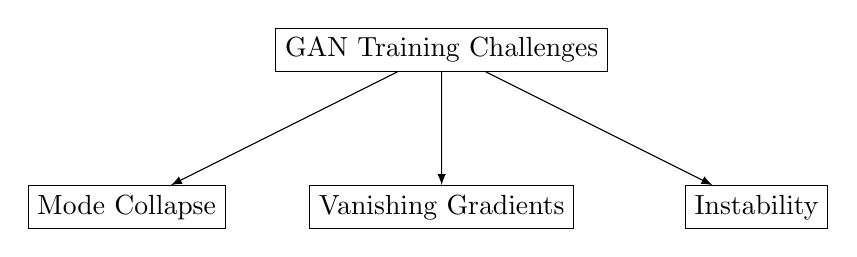
\begin{tikzpicture}[level distance=2cm, sibling distance=4cm, edge from parent/.style={draw,-latex}]
  \node[rectangle, draw] {GAN Training Challenges}
    child {node[rectangle, draw] {Mode Collapse}}
    child {node[rectangle, draw] {Vanishing Gradients}}
    child {node[rectangle, draw] {Instability}};
\end{tikzpicture}
\end{center}
\begin{itemize}
    \item \textbf{Feature Matching}: Instead of trying to fool the discriminator, the generator can be trained to match the intermediate features of the real and fake data produced by the discriminator. This can lead to more diverse and realistic samples~\cite{gui2021review}.
    \item \textbf{Progressive Growing}: This technique involves starting with a small model (low resolution) and gradually increasing the model size and resolution as training progresses. It helps GANs learn high-resolution images efficiently~\cite{karras2017progressive}.
    \item \textbf{Noise Injection}: Adding noise to the inputs of the discriminator or generator can help regularize the model, making it less sensitive to small variations in the data, and can improve the generalization of the network~\cite{hoff2002latent}.
\end{itemize}
